% Options for packages loaded elsewhere
\PassOptionsToPackage{unicode}{hyperref}
\PassOptionsToPackage{hyphens}{url}
\PassOptionsToPackage{dvipsnames,svgnames,x11names}{xcolor}
%
\documentclass[
  letterpaper,
  DIV=11,
  numbers=noendperiod]{scrartcl}

\usepackage{amsmath,amssymb}
\usepackage{lmodern}
\usepackage{iftex}
\ifPDFTeX
  \usepackage[T1]{fontenc}
  \usepackage[utf8]{inputenc}
  \usepackage{textcomp} % provide euro and other symbols
\else % if luatex or xetex
  \usepackage{unicode-math}
  \defaultfontfeatures{Scale=MatchLowercase}
  \defaultfontfeatures[\rmfamily]{Ligatures=TeX,Scale=1}
\fi
% Use upquote if available, for straight quotes in verbatim environments
\IfFileExists{upquote.sty}{\usepackage{upquote}}{}
\IfFileExists{microtype.sty}{% use microtype if available
  \usepackage[]{microtype}
  \UseMicrotypeSet[protrusion]{basicmath} % disable protrusion for tt fonts
}{}
\makeatletter
\@ifundefined{KOMAClassName}{% if non-KOMA class
  \IfFileExists{parskip.sty}{%
    \usepackage{parskip}
  }{% else
    \setlength{\parindent}{0pt}
    \setlength{\parskip}{6pt plus 2pt minus 1pt}}
}{% if KOMA class
  \KOMAoptions{parskip=half}}
\makeatother
\usepackage{xcolor}
\setlength{\emergencystretch}{3em} % prevent overfull lines
\setcounter{secnumdepth}{-\maxdimen} % remove section numbering
% Make \paragraph and \subparagraph free-standing
\ifx\paragraph\undefined\else
  \let\oldparagraph\paragraph
  \renewcommand{\paragraph}[1]{\oldparagraph{#1}\mbox{}}
\fi
\ifx\subparagraph\undefined\else
  \let\oldsubparagraph\subparagraph
  \renewcommand{\subparagraph}[1]{\oldsubparagraph{#1}\mbox{}}
\fi


\providecommand{\tightlist}{%
  \setlength{\itemsep}{0pt}\setlength{\parskip}{0pt}}\usepackage{longtable,booktabs,array}
\usepackage{calc} % for calculating minipage widths
% Correct order of tables after \paragraph or \subparagraph
\usepackage{etoolbox}
\makeatletter
\patchcmd\longtable{\par}{\if@noskipsec\mbox{}\fi\par}{}{}
\makeatother
% Allow footnotes in longtable head/foot
\IfFileExists{footnotehyper.sty}{\usepackage{footnotehyper}}{\usepackage{footnote}}
\makesavenoteenv{longtable}
\usepackage{graphicx}
\makeatletter
\def\maxwidth{\ifdim\Gin@nat@width>\linewidth\linewidth\else\Gin@nat@width\fi}
\def\maxheight{\ifdim\Gin@nat@height>\textheight\textheight\else\Gin@nat@height\fi}
\makeatother
% Scale images if necessary, so that they will not overflow the page
% margins by default, and it is still possible to overwrite the defaults
% using explicit options in \includegraphics[width, height, ...]{}
\setkeys{Gin}{width=\maxwidth,height=\maxheight,keepaspectratio}
% Set default figure placement to htbp
\makeatletter
\def\fps@figure{htbp}
\makeatother

\KOMAoption{captions}{tableheading}
\makeatletter
\makeatother
\makeatletter
\makeatother
\makeatletter
\@ifpackageloaded{caption}{}{\usepackage{caption}}
\AtBeginDocument{%
\ifdefined\contentsname
  \renewcommand*\contentsname{Table of contents}
\else
  \newcommand\contentsname{Table of contents}
\fi
\ifdefined\listfigurename
  \renewcommand*\listfigurename{List of Figures}
\else
  \newcommand\listfigurename{List of Figures}
\fi
\ifdefined\listtablename
  \renewcommand*\listtablename{List of Tables}
\else
  \newcommand\listtablename{List of Tables}
\fi
\ifdefined\figurename
  \renewcommand*\figurename{Figure}
\else
  \newcommand\figurename{Figure}
\fi
\ifdefined\tablename
  \renewcommand*\tablename{Table}
\else
  \newcommand\tablename{Table}
\fi
}
\@ifpackageloaded{float}{}{\usepackage{float}}
\floatstyle{ruled}
\@ifundefined{c@chapter}{\newfloat{codelisting}{h}{lop}}{\newfloat{codelisting}{h}{lop}[chapter]}
\floatname{codelisting}{Listing}
\newcommand*\listoflistings{\listof{codelisting}{List of Listings}}
\makeatother
\makeatletter
\@ifpackageloaded{caption}{}{\usepackage{caption}}
\@ifpackageloaded{subcaption}{}{\usepackage{subcaption}}
\makeatother
\makeatletter
\@ifpackageloaded{tcolorbox}{}{\usepackage[many]{tcolorbox}}
\makeatother
\makeatletter
\@ifundefined{shadecolor}{\definecolor{shadecolor}{rgb}{.97, .97, .97}}
\makeatother
\makeatletter
\makeatother
\ifLuaTeX
  \usepackage{selnolig}  % disable illegal ligatures
\fi
\IfFileExists{bookmark.sty}{\usepackage{bookmark}}{\usepackage{hyperref}}
\IfFileExists{xurl.sty}{\usepackage{xurl}}{} % add URL line breaks if available
\urlstyle{same} % disable monospaced font for URLs
\hypersetup{
  pdftitle={Animal Detection},
  colorlinks=true,
  linkcolor={blue},
  filecolor={Maroon},
  citecolor={Blue},
  urlcolor={Blue},
  pdfcreator={LaTeX via pandoc}}

\title{Animal Detection}
\author{}
\date{}

\begin{document}
\maketitle
\ifdefined\Shaded\renewenvironment{Shaded}{\begin{tcolorbox}[breakable, enhanced, boxrule=0pt, interior hidden, frame hidden, sharp corners, borderline west={3pt}{0pt}{shadecolor}]}{\end{tcolorbox}}\fi

Presentation by: Chris, Grant, Will

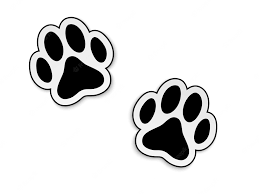
\includegraphics[width=\textwidth,height=3.64583in]{paws.png}

\hypertarget{background}{%
\subsection{Background}\label{background}}

Image classification is the process of assigning a label or class to an
input image based on its visual content. It is a fundamental task in the
field of computer vision and has a wide range of applications, including
object recognition, face detection, self-driving cars, and medical
imaging.

The importance of image classification stems from its ability to enable
machines to understand and interpret the visual world in the same way
that humans do. This capability can be used to automate various tasks,
such as identifying objects in an image, detecting and diagnosing
diseases in medical images, and enabling self-driving cars to navigate
safely. Additionally, image classification can be used to improve the
accuracy of other computer vision tasks, such as object detection and
segmentation.

With the increasing amount of visual data being generated and the
advancement of deep learning techniques, the field of image
classification has seen significant progress in recent years. This has
led to the development of highly accurate image classifiers that can be
trained on large datasets, and are able to generalize well to new
images.

\begin{figure}

{\centering 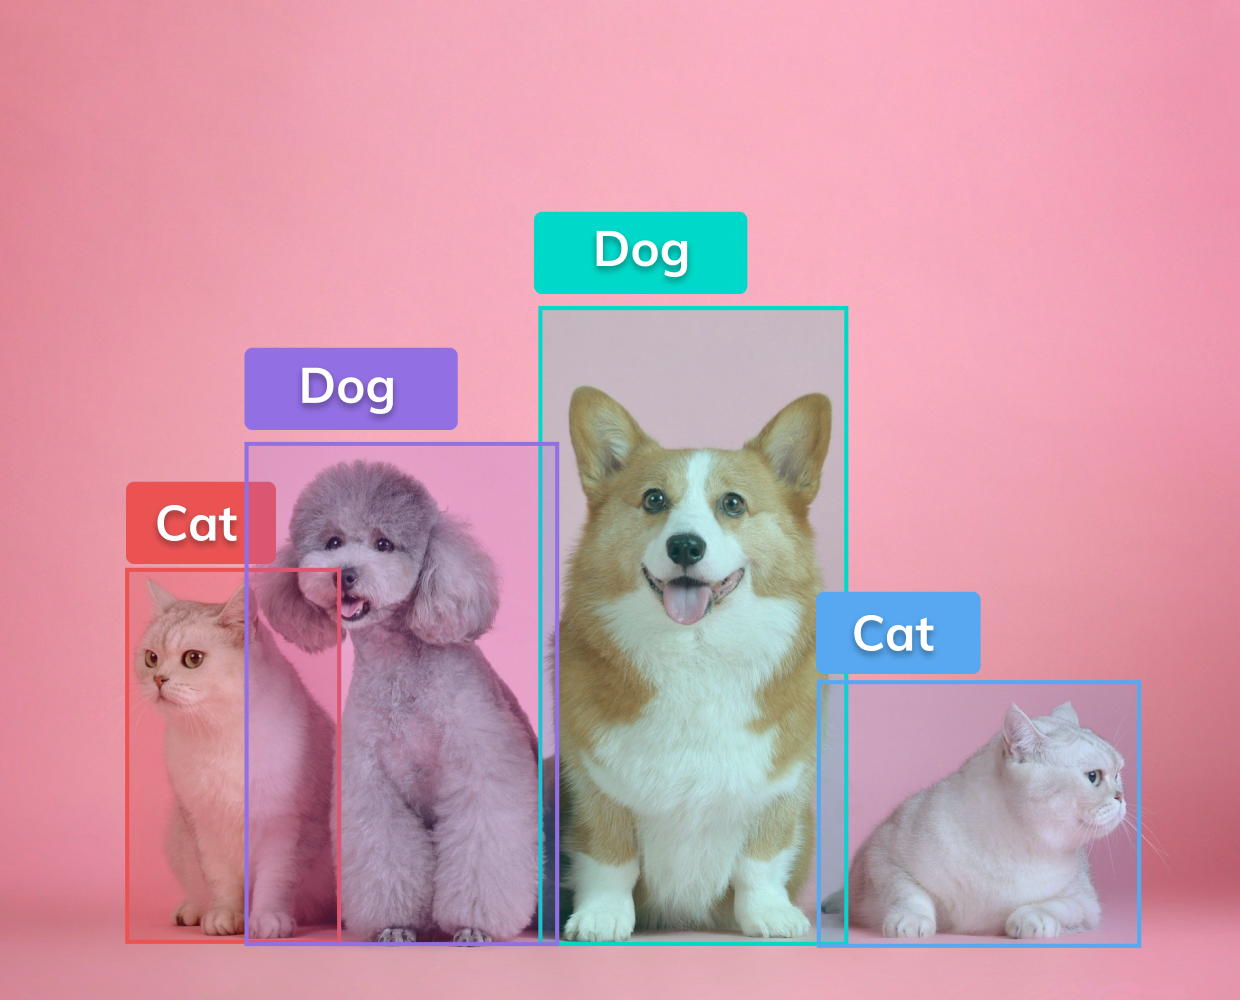
\includegraphics{animals.png}

}

\end{figure}

\hypertarget{question}{%
\subsection{Question}\label{question}}

Can we build a model that succesfully classifies the images of animals?

\hypertarget{exploratory-data-analysis}{%
\subsection{Exploratory Data Analysis}\label{exploratory-data-analysis}}

Our data is composed of 7 classes with over 1000 images

\begin{itemize}
\tightlist
\item
  Dogs
\item
  Elephants
\item
  Spiders
\item
  Chickens
\item
  Squirrels
\item
  Wolves
\item
  Butterflies
\item
  Horses
\end{itemize}

\hypertarget{data-cleaning-and-preparing-for-model}{%
\subsubsection{Data Cleaning and Preparing for
Model}\label{data-cleaning-and-preparing-for-model}}

\begin{itemize}
\item
  Each Image was resized to 150x150
\item
  All the images were then given their own label , and converted into an
  array
\item
  All labels were then one hot encoded.
\item
  We then used a 75\% traning set , 15\% validation set , and 10\% set
  split.
\end{itemize}

\hypertarget{methods}{%
\subsection{Methods}\label{methods}}

CNN

A convolutional neural network (CNN) is a type of deep learning model
that is commonly used for image and video analysis. It is called
``convolutional'' because it uses a technique called convolution to
analyze the data. In a CNN, the model learns to recognize patterns and
features in images by analyzing small sections (or ``patches'') of the
image at a time, and then combining the information from these patches
to understand the overall image. This makes CNNs well-suited for tasks
such as image classification, object detection, and image segmentation.

VGG16 model (CNN)

\begin{itemize}
\tightlist
\item
  13 convolutional layers
\item
  5 max pooling layers
\item
  3 fully connected layers
\item
  GlobalAveragePooling2D() layer
\item
  Dropout(0.2) layer
\item
  Dense(1024, activation=`relu') layer
\item
  Dropout(0.2) layer
\item
  Dense(6, activation=`softmax') layer as the final output layer.
\end{itemize}

So in total, it's 13 convolutional layers, 5 max pooling layers, 3 dense
layers and 2 dropout layers.

The model is trained on the ImageNet dataset, which contains millions of
images and thousands of object categories. Because of this, the model
has learned rich feature representations for a wide variety of
image-based tasks.

\begin{figure}

\begin{minipage}[b]{0.50\linewidth}

{\centering 

\raisebox{-\height}{

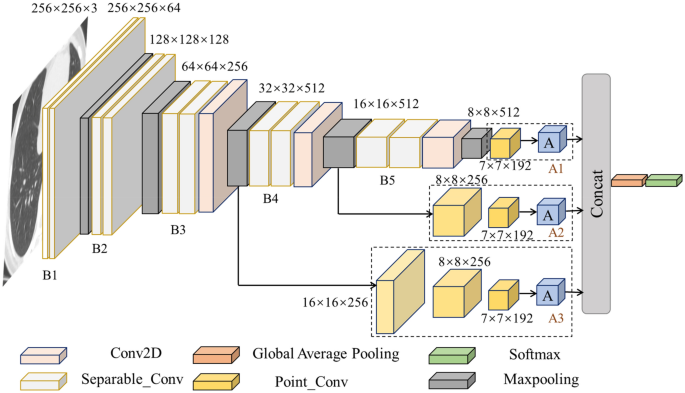
\includegraphics{CNN.png}

}

\caption{Convolutional Neural Network (CNN)}

}

\end{minipage}%
%
\begin{minipage}[b]{0.50\linewidth}

{\centering 

\raisebox{-\height}{

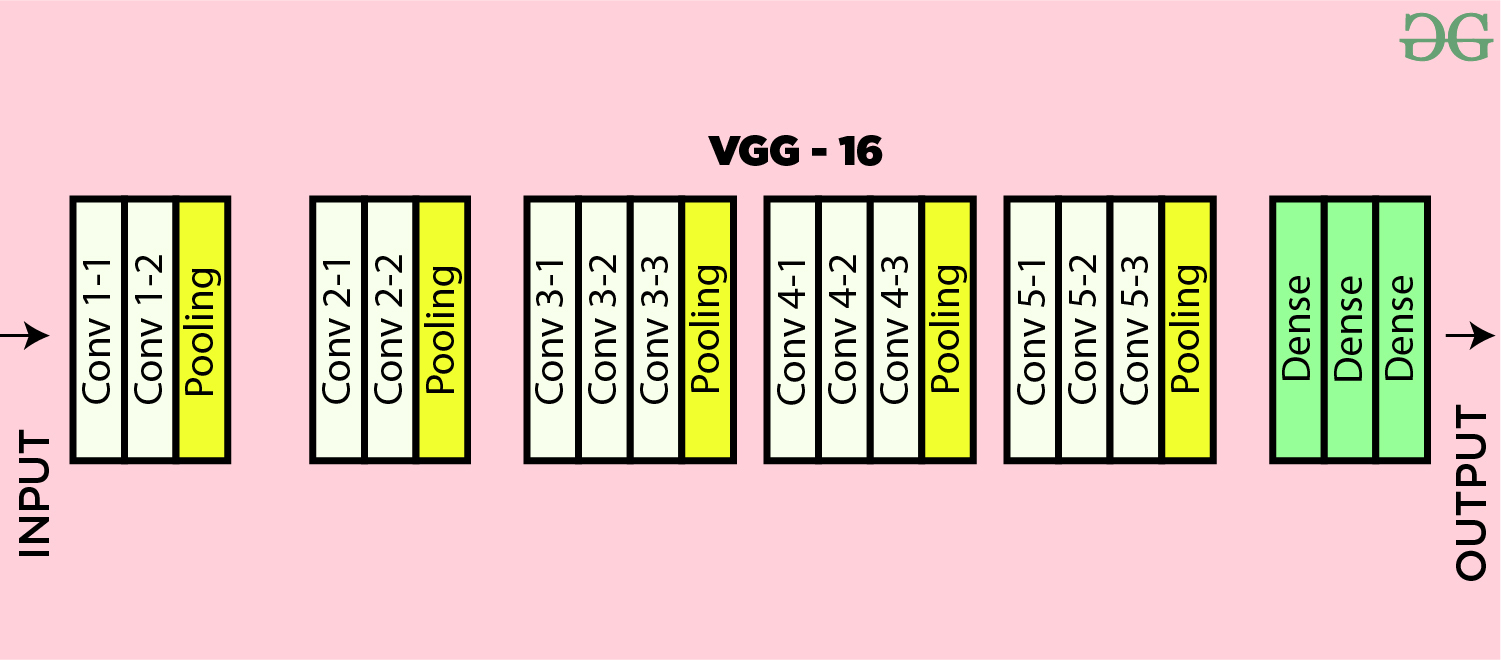
\includegraphics{VGG16.png}

}

\caption{VGG16 Model}

}

\end{minipage}%

\end{figure}

\hypertarget{evaluation}{%
\subsection{Evaluation}\label{evaluation}}

As seen in the table below the pretrain VGG model was able to perform
significanlty better than our own model. In practice using pretrained
models is the way to go and makes life so much easier.

\begin{verbatim}
        Model  Train Validation   Test
0  Team 6 CNN    99%        40%  32.2%
1       VGG16  97.7%      97.7%  91.2%
\end{verbatim}

Reasons our model did not perform well:

\begin{itemize}
\item
  Lack of sufficient data: With a small dataset, the model may learn to
  memorize the training data, which can lead to overfitting.
\item
  Complex architecture: A complex model with a large number of
  parameters may have the capacity to memorize the training data, which
  can lead to overfitting.
\item
  High learning rate: A high learning rate can cause the model to
  quickly adapt to the training data, which can lead to overfitting if
  the model does not have time to converge.
\item
  Lack of regularization: Regularization techniques such as dropout, L1,
  and L2 regularization can help prevent overfitting by adding a penalty
  to the model for having too many parameters.
\end{itemize}

Reasons VGG16 performs well:

\begin{itemize}
\item
  Deep architecture: VGG16 is a very deep model, with 16 layers, which
  allows it to learn a complex set of features from the input images.
  This depth enables the model to extract high-level features from the
  images, such as edges and shapes, which are important for image
  classification.
\item
  Small convolutional filters: VGG16 uses small convolutional filters
  (3x3) which enables the model to learn a large number of feature maps.
  This makes the model more expressive and able to capture fine-grained
  details in the images.
\item
  Max pooling: VGG16 uses max pooling layers which reduces the spatial
  dimension of the feature maps, making the model more robust to small
  translations of the objects in the images.
\item
  Large number of parameters: VGG16 has a large number of parameters,
  which enables it to learn a complex set of features from the images.
\item
  Pre-training: VGG16 was pre-trained on a large dataset (ImageNet),
  which means that it has already learned many useful features that can
  be used for other tasks.
\item
  ReLU activation: ReLU activation function is used in the model, which
  allows the network to learn non-linear decision boundaries, which
  helps to improve the performance of the model. VGG16 just does a much
  better job in detecting features especially since it has seen millions
  of similiar photos to ours.
\end{itemize}

The metric we will be using to evaluate our model is the accuracy.

\begin{figure}

\begin{minipage}[b]{0.50\linewidth}

{\centering 

\raisebox{-\height}{

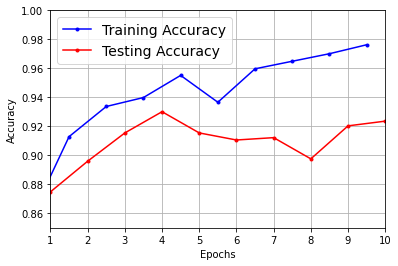
\includegraphics{Accuracy.png}

}

\caption{Accuracy}

}

\end{minipage}%
%
\begin{minipage}[b]{0.50\linewidth}

{\centering 

\raisebox{-\height}{

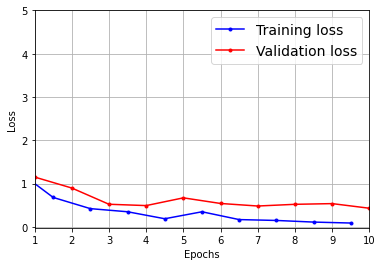
\includegraphics{Loss.png}

}

\caption{Loss}

}

\end{minipage}%

\end{figure}

\hypertarget{conclusion}{%
\subsection{Conclusion}\label{conclusion}}

We were able to succesfully build a model that classifies animals. We
achieved this through a VGG16 model that performed at a 91\% accuracy
compared to ours that did 30\%. This is a 61\% difference and 200\%
increase. Thus our model was two-times better.

CNN models are changing the world in many aspects including:

\begin{itemize}
\item
  Computer Vision: CNNS are used in a wide range of applications such as
  object detection, image classification, and image segmentation. These
  models are used in self-driving cars, security systems, and robotics.
\item
  Medical imaging: CNNs are used in medical imaging to improve the
  accuracy of diagnoses and to detect diseases such as cancer and heart
  disease.
\item
  Natural Language Processing: CNNs are used in natural language
  processing (NLP) to analyze text and speech, which has applications in
  language translation, text summarization, and sentiment analysis.
\item
  Recommender systems: CNNs are used in recommender systems to make
  personalized recommendations to users based on their past behavior and
  preferences.
\item
  Generative models: CNNs are used to generate new images, videos and
  audio, which have applications in art, entertainment, and
  communication.
\item
  Robotics: CNNs are used in robotics to help the robots understand and
  interact with their environment, they can be used for tasks such as
  grasping and manipulation.
\end{itemize}

CNNs have the potential to revolutionize many industries and improve the
lives of many people by making tasks more efficient, accurate and
faster. However, it's important to keep in mind that these models are
not perfect and may have limitations and biases, and it's important to
address these issues to ensure fair and ethical use of these models.

\hypertarget{sources}{%
\subsection{Sources}\label{sources}}

Very Deep Convolutional Networks for Large-Scale Image Recognition, K.
Simonyan and A. Zisserman. arXiv:1409.1556.
https://neurohive.io/en/popular-networks/vgg16/
https://arxiv.org/abs/1409.1556
https://www.robots.ox.ac.uk/\textasciitilde vgg/research/very\_deep/
https://github.com/keras-team/keras-applications/blob/master/keras\_applications/vgg16.py



\end{document}
